
\documentclass[11pt]{article}
\usepackage{amsmath,amssymb}
\usepackage{graphicx}
\usepackage{natbib}
\usepackage[parfill]{parskip}
\usepackage[margin=1in]{geometry}
\usepackage{pdflscape}
\title{Supplementary information for ``CLM5-PPE"}
\author{D. Kennedy}
\renewcommand{\thefigure}{S\arabic{figure}}
\begin{document}
\maketitle

\begin{figure}[h]
\centering
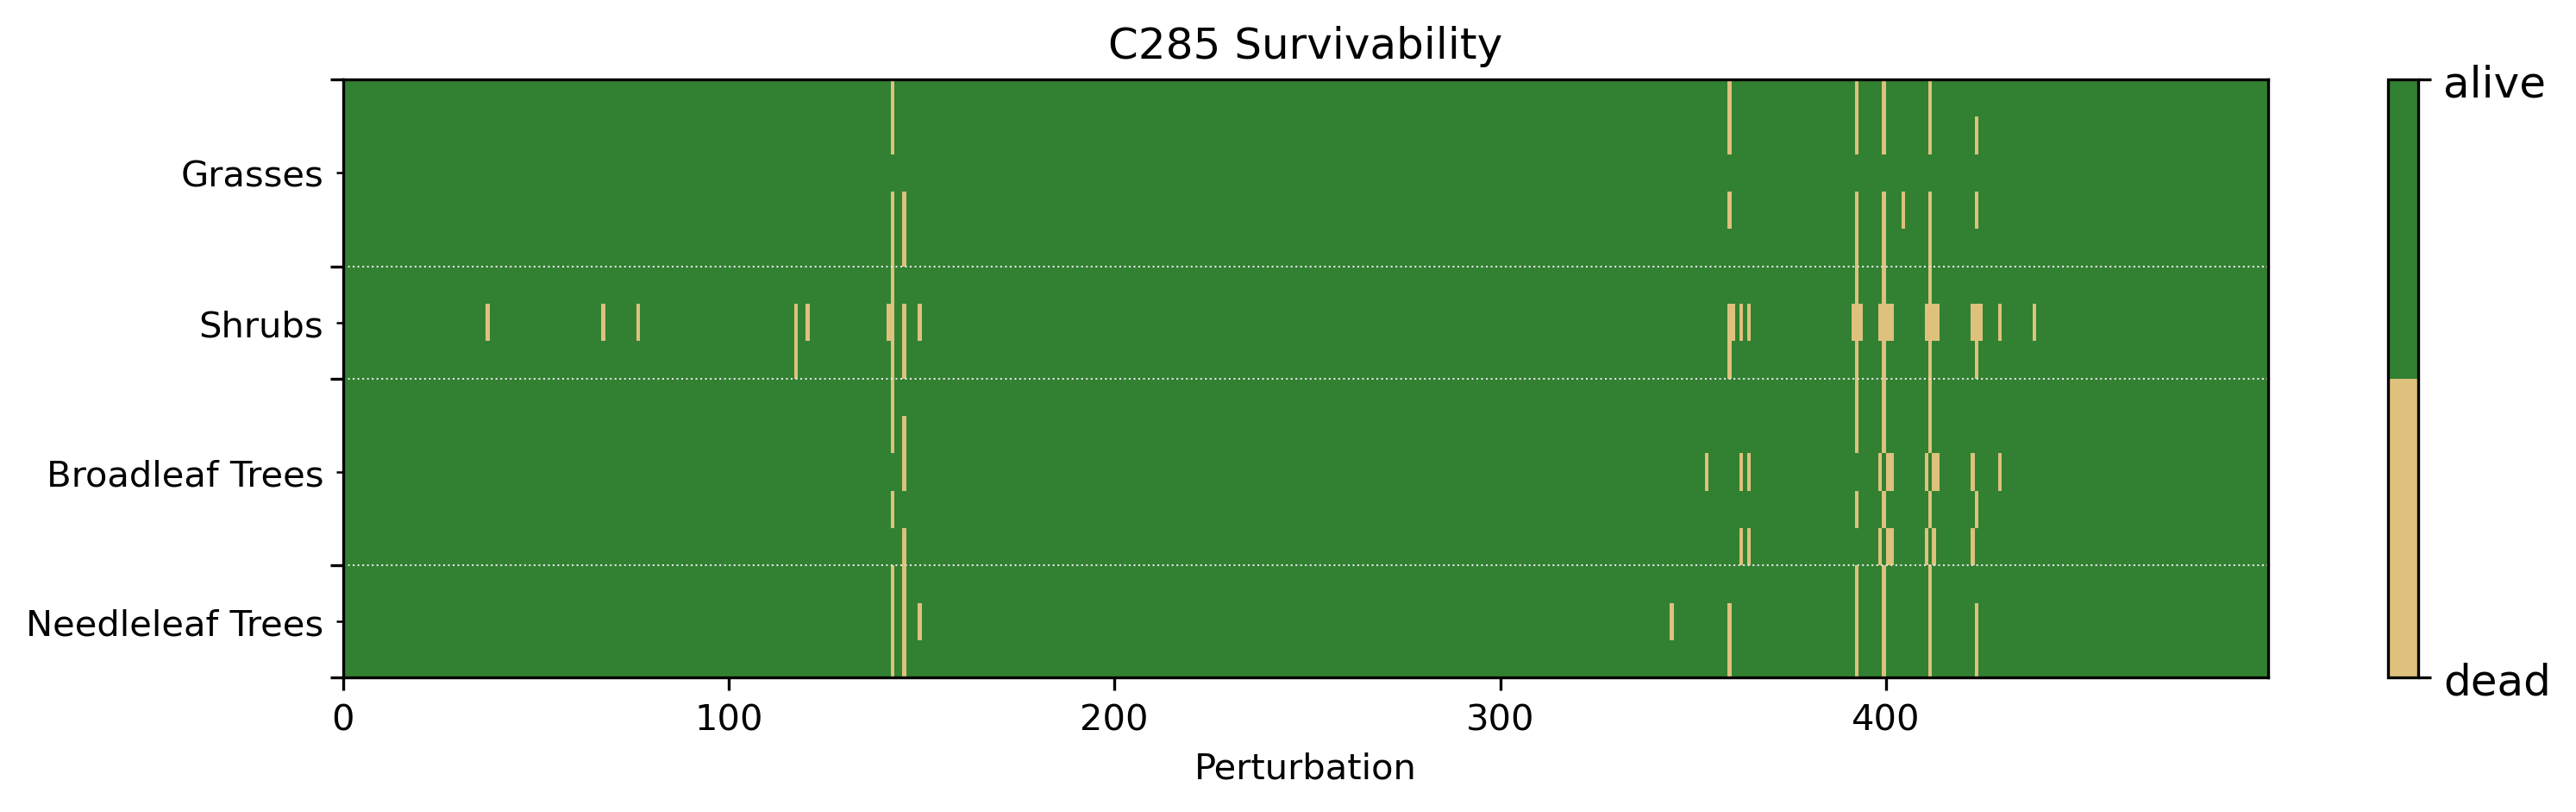
\includegraphics[width=\textwidth]{figs/supp/survivability_c285.png}
\caption{Survivability.}
\label{supp:surv}
\end{figure}

\begin{landscape}
\begin{figure}[h]
\centering
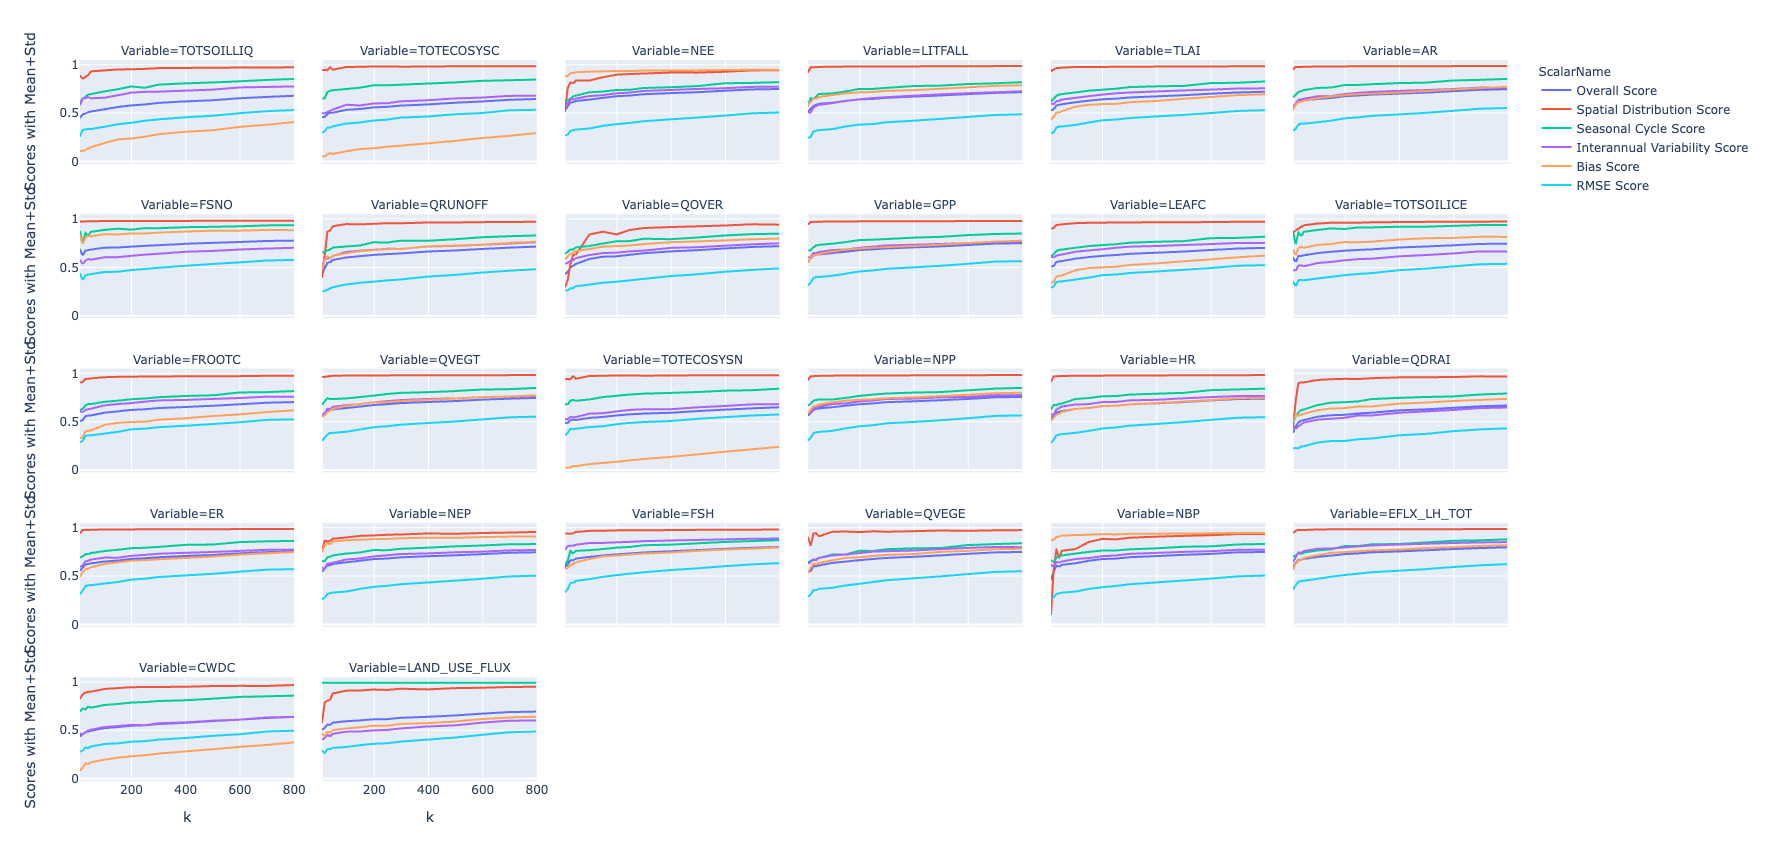
\includegraphics[width=60pc]{figs/supp/ilamb_lines.png}
\caption{The convergence of several scoring metrics with increasing sparsegrid resolution across a variety of CLM variables. All scores tend towards 1 as the number of sparsegrid clusters (k) approaches the 5666 gridcells for the native resolution of our 2-degree simulations. }
\label{supp:ilamb}
\end{figure}
\end{landscape}

\end{document}
